\section{System Design}
\subsection{Subsystem Identification}
The subsystems of this project are broken up base on their function and dependencies, this is as follows: Editor Subsystem, Chess Subsystem, Board Subsystem, AI Subsystem*, Authentication Subsystem*, Network Play Subsystem*, Statistics Subsystem, and Lobby Subsystem*.

The Editor and Chess subsystems both depend on the Board subsystem, but have functionality that are distinctly different in purpose; latter having rules and turns while the former has has the ability to manipulate the board without such constraints.

The Authentication, Network Play, and Lobby subsystems* are dependent on the web server. There is a distinct flow from authentication to lobby to network play.

Statistics subsystem has its own unique requirements for storing the data that needs to be addressed.

AI Subsystem is optional, and while works with the chess subsystem, is not always there so should be considered as a separate system.

\paragraph{Chess Gameplay}
\subsection{Subsystem Communication}
\paragraph{Game Subsystems}
The game subsystems (AI*, Chess, Editor, Board) have minimal interaction with other subsystems. When they are in use, events from the board are passed to either the chess or editor subsystem to be processed and the outcome is given to the board. The AI subsystem will interact with the chess subsystem when the players turn has ended, which it will be given a FEN string, and return a FEN string with its move.

\paragraph{Network Subsystems}
These subsystems as mentioned earlier, have a flow to them in which authentication leads into the lobby subsystem which leads to the network play subsystem. 

\subparagraph{Account Creation Management}
The user will modify their account information via the Chess Game UI that will be fed into their respective records in the database.

\subparagraph{Chess Gameplay Management}
Gameplay metrics will be automatically tracked by the Chess Game UI in tandem with pre-existing records stored in the MySQL database. Gameplay involving the computer will be handled by the StockFish AI program to determine the next best move.
\paragraph{Statistics Subsystem}
This subsystem is unique in that it has its own unique interactions with the Chess Subsystem and the Authentication subsystem.

\subsection{Diagrams}
\begin{center}
	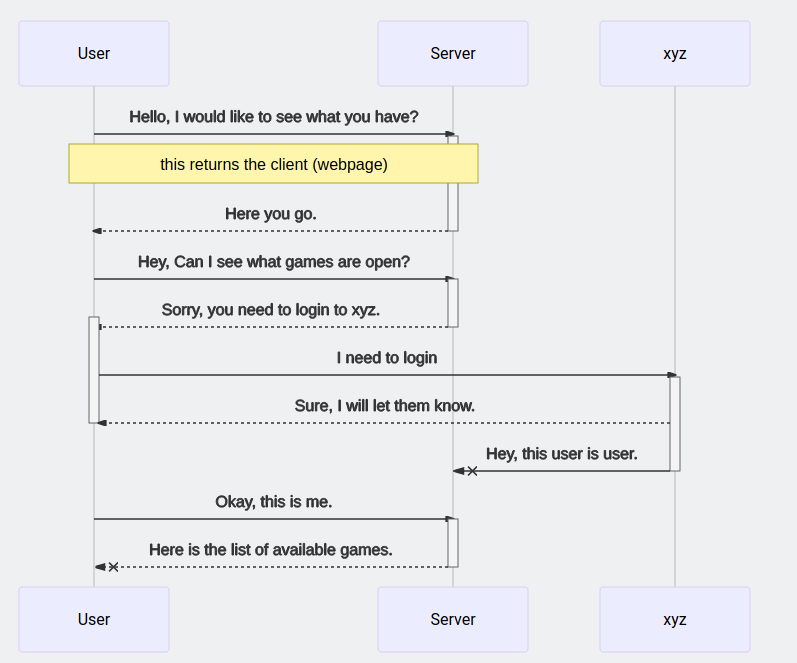
\includegraphics[width=.9\linewidth]{../diagrams/out/Sequence1.png}
\end{center}
\begin{center}
	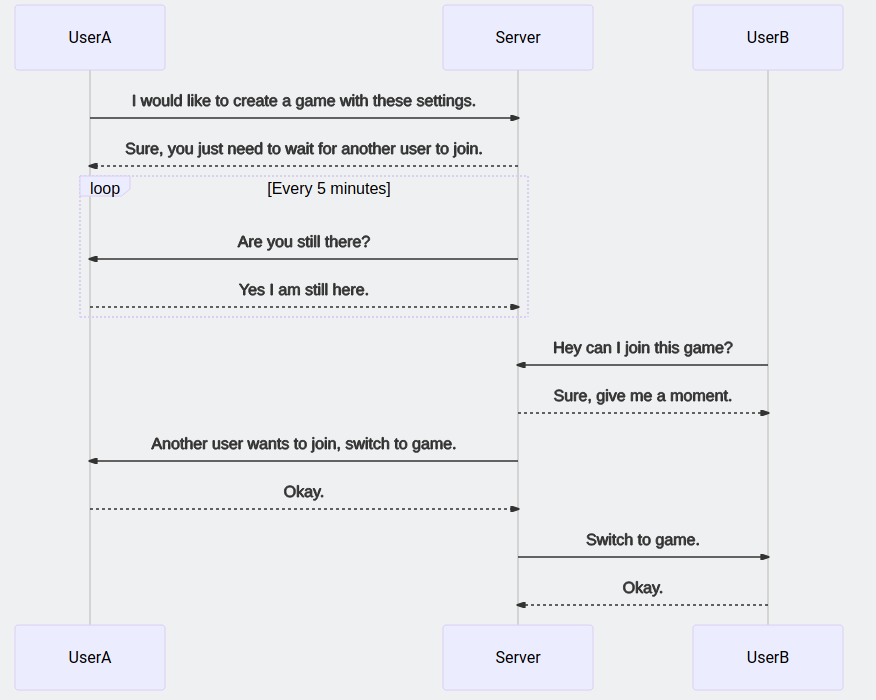
\includegraphics[width=.9\linewidth]{../diagrams/out/Sequence2.png}
\end{center}
\begin{center}
	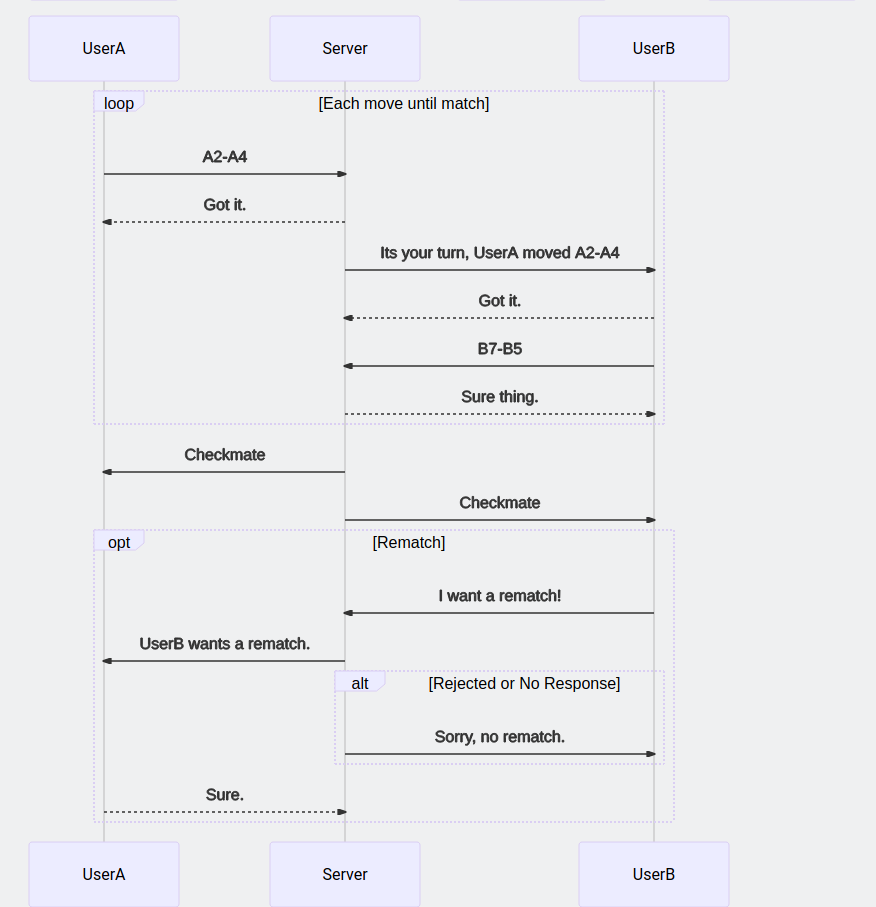
\includegraphics[width=.9\linewidth]{../diagrams/out/Sequence3.png}
\end{center}
\begin{center}
	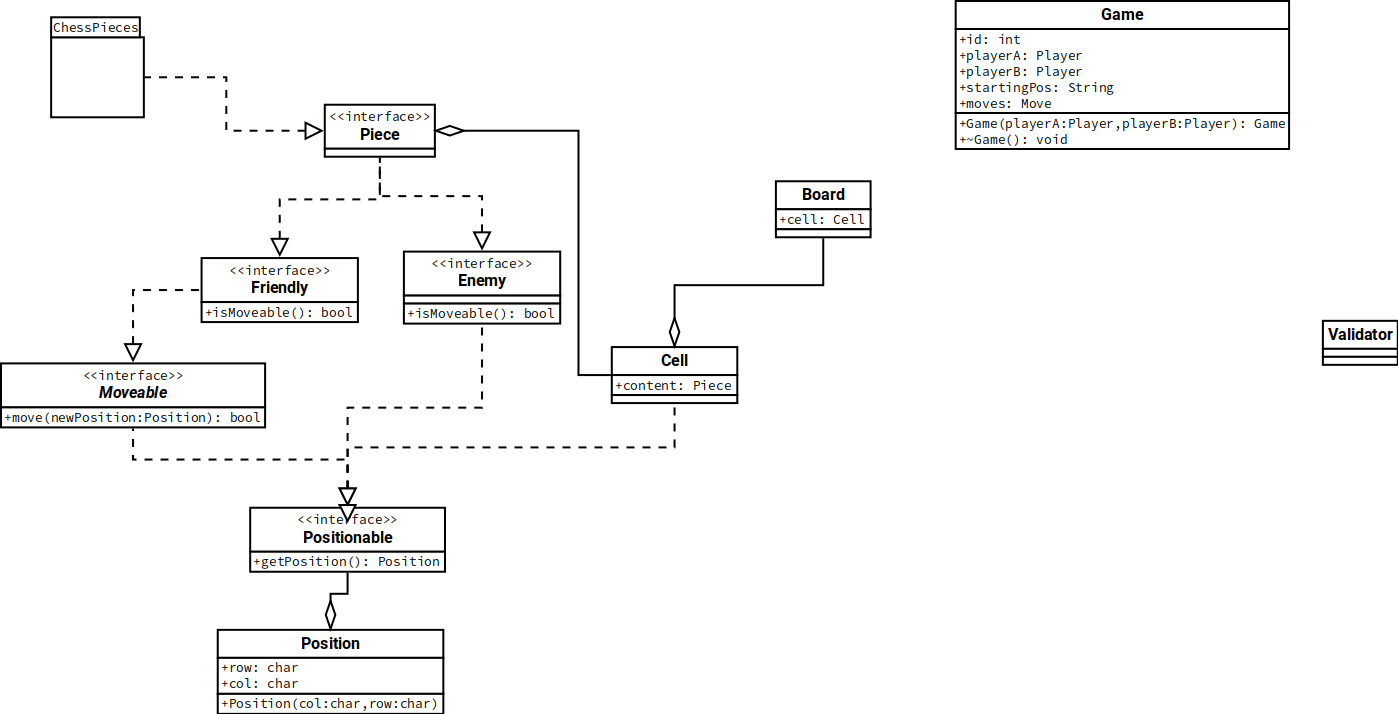
\includegraphics[width=.9\linewidth]{../diagrams/out/ClassDiagram.png}
\end{center}
\begin{center}
	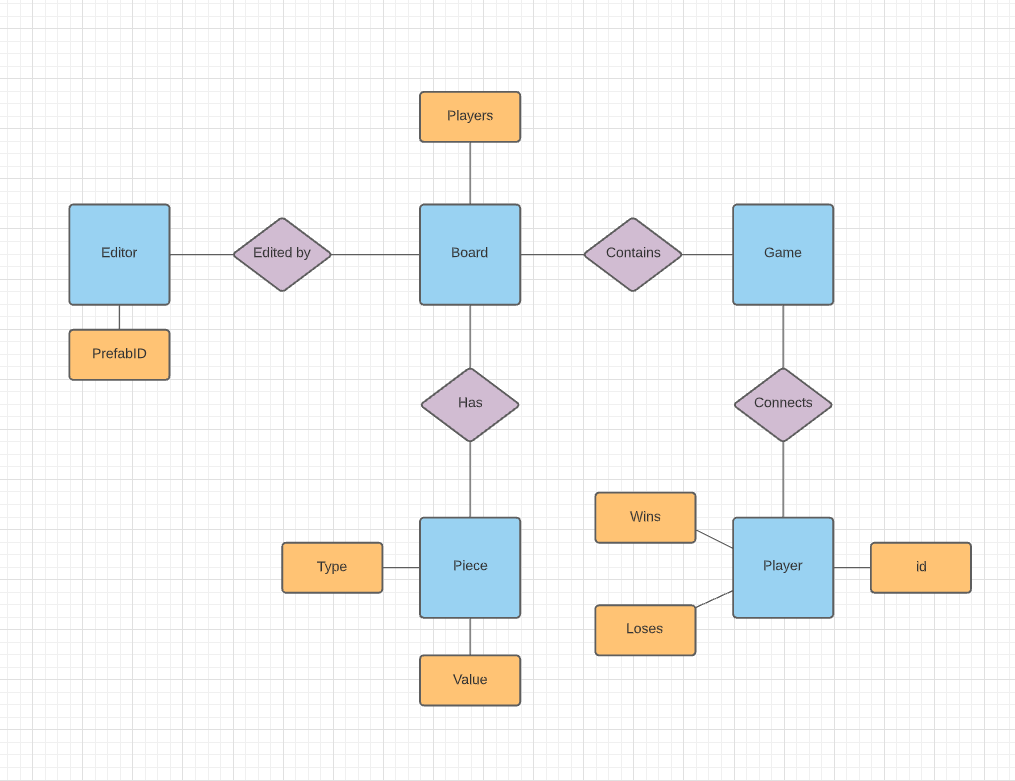
\includegraphics[width=.9\linewidth]{../diagrams/out/ERDiagram.png}
\end{center}